\begin{center}
    \Large{\textbf{Теоретична частина}}    
\end{center}

\vspace{1mm}

В роботіпропонується використати деякі оптичні схеми, за допомогою
яких формується два джерела когерентного випромінювання, інтерференцію від
яких можна спостерігати на екрані.

\begin{wrapfigure}{l}{0.5\textwidth}
    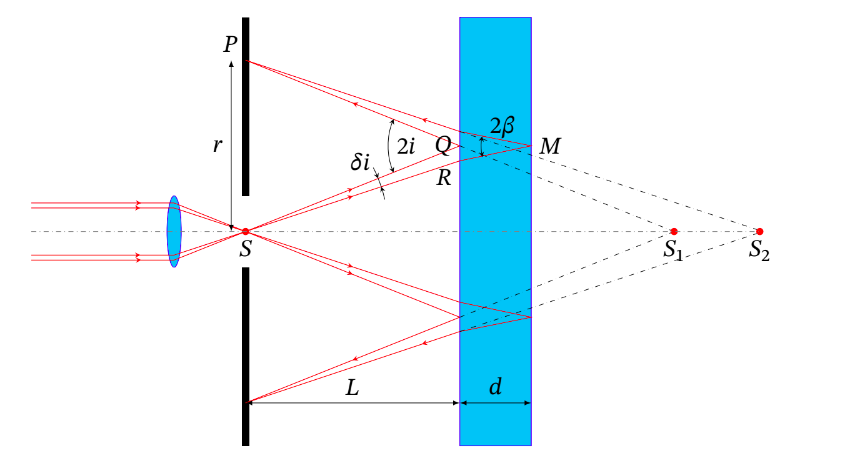
\includegraphics[width=0.5\textwidth]{assets/main_scheme.png}
    \caption{Схема роботи}
\end{wrapfigure}

На рис. 1 зображено схему, в якій за допомогою скляної 
платівки утворюється два уявних джерела когерентного світла.
Світловий промінь 2 від лазера 1 проходить крізь короткофокусну лінзу 3,
змонтовану в центрі екрана 4. Процес розсіяння світла лінзою
можна розглядати як утворення уявного точкового джерела
когерентного випромінювання $S_0$. Внаслідок подальшого відбиття
світла від передньої та задньої поверхні поверхні платівки 
утворюється два уявних точкових джерела $S_1$, $S_2$ світло
яких інтерферує на поверхні екрана 4. Для отримання чіткої інтерференційної
картини з максимальним освітленням в центрі екрана необхідно, щоб
джерела $S_0$, $S_1$, $S_2$ містились на одній прямій. Промінь 2 має попадати
точно в центр лінзи. Екран 4 та платівка 5 паралельні один
одному, що досянається за допомогою регулюючого гвинта на утримувачі платівки 5.


В наведеній схемі апертура інтерференції залежить від точки інтерференційного поля,
тобто від кута $\Theta$. Проте для малих кутів$\Theta$ цією залежнісю
можна знехтувати. Як видно з рис. 1,

\begin{equation}
    2 \omega = \frac{h}{L+l} \sin{2\Theta},
\end{equation}

де $h=\frac{h_0}{n}$ - оптична товщина платівки,
$L$  - відстань між платівкою та екраном,
$l = L - f$ - відстань між джерелом $S_0$ та екраном,
$f$ - фокусна відстань лінзи 3.

Відомо, що 

$$ B = \frac{L \lambda}{d} = \frac{\lambda}{2\omega} $$.

Тоді ширина інтерференційної смуги:

\begin{equation} \label{eq:2}
    B\Theta = \frac{\lambda(2L - f)\Theta}{h_0 \sin{2\Theta}}n \simeq 
    \frac{\lambda L}{h_0} n - \frac{f}{2 h_0}n 
\end{equation}

%\begin{figure}[h]    
%    \centering
%    \includegraphics[width=.7\textwidth]{assets/filename }
%    \caption{Підпис}
%\end{figure}